\documentclass[prodmode,acmtrets]{acmsmall}
\usepackage{algorithm}
\usepackage{algorithmic}
\usepackage[algo2e]{algorithm2e}
\renewcommand{\algorithmcfname}{ALGORITHM}
\SetAlFnt{\small}
\SetAlCapFnt{\small}
\SetAlCapNameFnt{\small}
\SetAlCapHSkip{0pt}
\IncMargin{-\parindent}

% Metadata Information
\acmVolume{0}
\acmNumber{0}
\acmArticle{1}
\acmYear{2014}
\acmMonth{0}

\usepackage{graphicx}
\usepackage{multirow}
\usepackage[caption=false,font=footnotesize]{subfig}
\usepackage{dblfloatfix}
\usepackage{xspace}
\usepackage{url}
\usepackage[square, comma, sort&compress, numbers]{natbib}

\setlength{\parskip}{0pt}
\renewcommand{\topfraction}{1}
\renewcommand{\textfraction}{0.15}
\renewcommand{\dbltopfraction}{1}

\renewcommand\floatpagefraction{.9}
\renewcommand\topfraction{.9}
\renewcommand\bottomfraction{.9}
\renewcommand\dbltopfraction{.9}
\renewcommand\textfraction{.1}   
\setcounter{totalnumber}{4}
\setcounter{topnumber}{8}
\setcounter{bottomnumber}{4}
\setcounter{dbltopnumber}{4}

\newcommand{\eqnref}[1]{(\ref{#1})}
\newcommand{\figref}[1]{Figure~\ref{#1}}
\newcommand{\algref}[1]{Algorithm~\ref{#1}}
\newcommand{\secref}[1]{Section~\ref{#1}}
\newcommand{\tabref}[1]{Table~\ref{#1}}

\newcommand{\tabincell}[2]{\begin{tabular}{@{}#1@{}}#2\end{tabular}}

\graphicspath{{./figures/}}

\begin{document}

\markboth{C.Liu et al.}{QuickDough: A Rapid FPGA Accel. Design Framework using SCGRA Overlay}

\title{QuickDough: A Rapid FPGA Accelerator Design Framework using Soft Coarse-Grained Reconfigurable Array Overlay}
\author{CHENG LIU
\affil{The University of Hong Kong}
COLIN YU LIN
\affil{The University of Hong Kong}
HAYDEN KWOK-HAY SO
\affil{The University of Hong Kong}
}

\begin{abstract}
    With the advancement of the FPGA techniques and the increase of successful demonstrations 
of using FPGAs in data center, more and more cloud computing vendors start to integrate 
FPGAs as computing resources in the cloud. In order to make best use of the computing resources 
in the cloud, the computing resources are usually virtualized such that they can be shared by different 
computing tasks from either a single user or multiple users. Nevertheless, unlike the 
conventional computing resources such as CPUs and GPUs, FPGAs are difficult to be virtualized 
and shared at runtime for two reasons. On the one hand, the same FPGA design requires lengthy implementation 
targeting different types of FPGA devices and thus the same task can't be migrated to 
a different type of FPGA device. On the other hand, 
CGRA overlay which is an intermedaite layer built on top of FPGAs can be shared by 
different applications and also allows efficient runtime context switch. Thus we explores 
CGRA overlay for the FPGA resource virtualization. 



The design productivity of FPGA development which remains magnitudes lower compared to typical software development severely hinders the widespread adoption of FPGAs. Particularly, the lengthy low-level FPGA implementation process including synthesis, placing and routing dramatically limits the number of compile-debug-edit cycles per day and lowers the FPGA design productivity. To address this design productivity problem, we have developed a rapid FPGA loop accelerator generation framework called QuickDough. Instead of trying to reduce the implementation time, it reuses a pre-built accelerator library to avoid the lengthy implementation process during design iterations. By utilizing a soft coarse-grained reconfigurable array (SCGRA) overlay built on top of off-the-shelf FPGAs as the backbone of the accelerators in the library, it compiles a high-level loop to the FPGA through a rapid operation scheduling first and then generates the FPGA accelerator bitstream through a rapid integration of the scheduling result and a pre-built accelerator bitstream selected from the library. According to the experiments, QuickDough is able to produce accelerators in the order of seconds while achieving up to 9X performance speedup over the execution of the same software running on a hard ARM processor.  

\end{abstract}

\terms{Design, FPGA, Overlay, CGRA}
\keywords{Overlay, FPGA Accelerator, Soft Coarse 
Grain Reconfigurable Array, Design Productivity}

\acmformat{Cheng Liu, Colin Yu Lin, and Hayden Kwok-Hay So, 2014. 
QuickDough: A Rapid FPGA Accelerator Design Methodology Using Soft 
Coarse-Grained Reconfigurable Array Overlay.}

\begin{bottomstuff}
This work is supported by xxx

Author's addresses: Cheng Liu, Colin Yu Lin, and Hayden Kwok-Hay So
Department of Electrical and Electronic Engineering, The University of
Hong Kong, Pokfulam Road, Hong Kong

\end{bottomstuff}

\maketitle

\section{Introduction}
Improving general-purpose processing system is getting extremely 
difficult. More and more computer architects believe that the major 
improvements in cost-energy-performance will come from domain-specific 
hardware accelerators. Recent years have already seen a number of successful 
demonstrations utilizing domain specific hardware accelerators for critical 
domains of applications such as deep neural network \cite{Jouppi2017tpu, Li2017survey} 
database operations \cite{Wu2014q100} and graph processing \cite{Jun2016graphicionado, Ozdal2016energy}. 
In order to explore the hardware accelerator design, a hardware accelerator simulator 
is usually required. Indeed there are already many exisitng tools \cite{systemc, chisel} and 
models \cite{dramsim2, ramulator} that can be used to help with the hardware accelerator 
design, it is non-trivial to develop a hardware accelerator on top of these work. For instance, there 
is a lack of general public cycle-accurate memory models available in \cite{systemc, chisel} while 
\cite{dramsim2, ramulator} expose only primitive memory access interface and need to be further 
wrapped for an accelerator simulator. And a general accelerator simulator 
framework is highly desired for the hardware accelerator simulator development.

Despite the difference of the accelerator simulators, we argue that a general 
accelerator simulator design framework should have three common yet important 
features. First of all, it should provide memory models of various memory 
architectures. Basically memory is usually critical to the hardware accelerator 
and greatly affects the accelerator design. At the same time, memory techniques evolve rapidly 
over the years and novel memory architectures with distinct features emerge. In order to explore 
hardware accelerator design, various memory architectures needs to be evaluated. 
Secondly, it should provide abstract user-frinedly memory interfaces. Hardware accelerators 
usually have complex memory access patterns such as stream access, burst access as well as random access. 
Thus higher abstract memory access interface instead of primitive memory access interface should be provided. 
Thirdly, it should provide trade-off between simulation speed and precision. Hardware accelerators 
may have distinct simulation speed and precision requirements while exploring the hardware accelerator. 
For instance, some of the applications such as graph accelerators may process on a big data set. 
Low-level accurate memory model may result in extremely long simulation. Thus a simplified memory model 
should be used to obtain the general performance of the accelerators. For applications that are sensitive 
to the memory access latency, more accurate memory models are preferred.

There is still a lack of general accelerator simulator framework that fullfills 
all the three features mentioned above. To that end, we proposed a flexible hardware accelerator 
simulation framework to be reused for general hardware accelerator simulator development. Basically, it 
integrates ramulator supporting various memory architectures as the underlying memory model and thus allows 
hardware accelerator exploration over a broad range of memory architectures. In addition, abstract memory 
interfaces as well as memory content management are provided to faciliate the accelerator accessing 
the memory model. Finally, it also provides a mix of cycle-accurate memory model and simiplified 
analytical memory model obtained though sampling to compromise on simulation speed and accuracy.

The rest of the paper is organized as follows. Section 2 is the realted work, Section 3 presents 
the proposed accelerator simulation framework. Section 4 provides the experimental results 
and Section 5 concludes this paper.






\section{Related Work} \label{sec:relatedwork}
Despite of the performance and power advantages, the design 
productivity of developing FPGA applications remains low 
due to the lengthy compilation and complex application-specific 
customization. And it has become the major obstacle 
that hinders the wide adoption of FPGAs as commodity computing devices. 
The community from both the industry and academia have developed 
many different methods from diverse angles to tackle the problem. 
These methods can be roughly classified into three categories. 
The first category mainly focuses on improving the low-level 
implementation tools. A number of approaches such as making 
quality/runtime trade-offs \cite{mulpuri2001runtime}, parallel 
compilation \cite{moctar2014parallel, goeders2011deterministic, altera-pc, 
xilinx-pc} and using hard-macro techniques \cite{lavin2013improving, 
korf2011automatic} have been explored from this angle. The second 
category mainly centers the HLS design flow while the third one 
primarily relies on the overlay concept. They later two categories 
will be detailed in the following sections.

\subsection{High-Level Synthesis} 
With many years of continuous endeavor, a number of tools have emerged as 
mature solutions for HLS \cite{VivadoHLS, Legup, zhang2008autopilot}. They typically 
allow designers to express hardware designs using high-level  
description languages such as C, C++ etc. and also enable evaluation of different 
design choices using pragmas or directives. Indeed, they significantly improve 
the design productivity compared to the conventional hardware design flow using 
hardware description languages. However, when considering the overall design 
productivity of developing hybrid software-gateware applications, HLS is 
only addressing part of the problem, as the lengthy low-level compilation 
including synthesis, mapping, placing and routing remains a bottleneck for 
an application designer \cite{ROB2014, capalija2014tile}.

Customizing the generated hardware specifically to an user 
application is also time-consuming for designers and thus critical to the design 
productivity. A number of algorithms such as generic algorithms 
relied on local-search techniques \cite{schafer2009adaptive, 
sengupta1997genetic}, learning-based methods \cite{onlinecustomization, 
carrion2012machine}, divide and conquer algorithm \cite{DCcustomization} 
and a calibration free algorithm \cite{RCcustomization} etc. have been developed 
to perform the DSE on top of HLS tools. The algorithms can efficiently help automate the 
customization or DSE process. However, the algorithms must rely on HLS tools 
to estimate the implementation information such as implementation frequency, 
overhead or power for the corresponding customization. While the hardware generated 
can be irregular and may vary dramatically, thus the accuracy of the estimation 
especially on implementation frequency and power can be rather limited, which may
fail to optimize an HW/SW co-design problem.  

\subsection{Overlay Architectures}
Overlay architecture which is a virtual intermediate architecture overlaid on 
top of off-the-shelf FPGA is increasingly applied as a way to address the 
productivity challenge. 

Various overlays with diverse configuration granularities and flexibility 
ranging from virtual FPGAs \cite{Grant2011Malibu, ZUMA2012}, 
array-of-FUs \cite{mesh-FUs,ferreira2011fpga}, soft 
CGRA \cite{kissler2006dynamically, scgra-orig}, soft GPU \cite{Guppy2012GPU-Like}, 
vector processors\cite{Yiannacouras2009FPS, MXP2013} to 
configurable processors or multi-core processors \cite{unnikrishnan2009application, 
MARC2010, Yiannacouras2007Exploration, Capalija2009coarse-grain, OCTAVO2012, iDEA2012} 
have been developed over the years. SCGRA overlay provides unique 
advantages on compromising hardware implementation 
and performance for compute intensive nested loops as demonstrated 
by numerous ASIC CGRAs \cite{tessier2001reconfigurable, compton2002reconfigurable}.
Most importantly, it allows both rapid compilation by taking advantage of 
the overlays' tiling structure \cite{ROB2014} and efficient bitstream 
reuse within the design iterations of an application \cite{scgra-orig}, 
thus it is particularly promising for high productivity nested loop acceleration.

Despite of the promising potential, a complete automatic customization 
framework that enables application-specific optimization is still highly 
anticipated for the sake of design productivity and performance. 
The authors in \cite{colinheart} developed an SCGRA topology customization method 
using genetic algorithm and showed the potential benefits of the SCGRA 
overlay customization. However, the rest system design parameters such as 
on chip buffer size, loop unrolling factor etc. are not covered. 

Indeed, SCGRA overlays have many similarities in terms of array structure 
and scheduling algorithm with ASIC CGRAs. Nevertheless, ASIC CGRAs emphasize 
more on configuration capability and limited customization is allowed due 
to the overhead constraints \cite{zhou2014application, miniskar2014retargetable} 
while SCGRA overlays allow more intensive architectural customization 
because of the FPGA's inherent programmability. Moreover, hardware resources such as 
DSP blocks and RAM blocks available on FPGAs are discrete, which results in different 
design constraints for SCGRA overlay customization as well. 

By utilizing the SCGRA overlay as the backbone of the FPGA accelerator, 
a complete nested loop acceleration framework 
targeting CPU-FPGA system is developed. It supports intensive application-specific
customization including the overlay architectural customization, 
the compilation customization and communication interface customization 
for various design goals. When the customized design parameters are determined, 
corresponding hardware accelerator and software can be compiled to the target 
CPU-FPGA system rapidly eventually providing a push-button solution for a nested loop 
acceleration. 



\section{Resilient training framework} \label{sec:framework}
Resilient neural networks allow significant performance or 
energy efficiency improvement with little prediction accuracy penalty 
by relaxing the neural network accelerator design constraints. 
This motivates us to obtain more resilient neural networks 
for advantageous accelerator design trade-offs. 
A resilient neural network training framework will be 
detailed in this section. 

\subsection{Overall training framework}
For the problem that the computing error patterns are 
difficult to be captured in training with GPPs, 
we have the accelerators with computing errors integrated into 
the training process. Forward processing influenced by 
the accelerator computing errors is used in training directly 
such that computing error patterns and application data are 
reflected in the neural network models. For the problem that 
some of the layers are affected more than the others, 
we take these layers as critical layers and opt to 
protect the layers from being affected by computing errors. 
With reasonable performance penalty, we can improve the 
overall neural network resilience. 

Following this idea, the overall training framework is depicted in Figure \ref{fig:retrain}. 
Instead of training on GPPs, it has the majority of forward computing performed on the 
accelerators with computing errors while the rest of the training remains on GPPs.
Note that the critical layers should be executed on reliable hardware 
while GPP is one of the options. There are many different approaches 
that can be used to relax the design constraints.
Although they may cause distinct computing errors, they can be fitted to the 
same training framework.

\begin{figure}
        \center{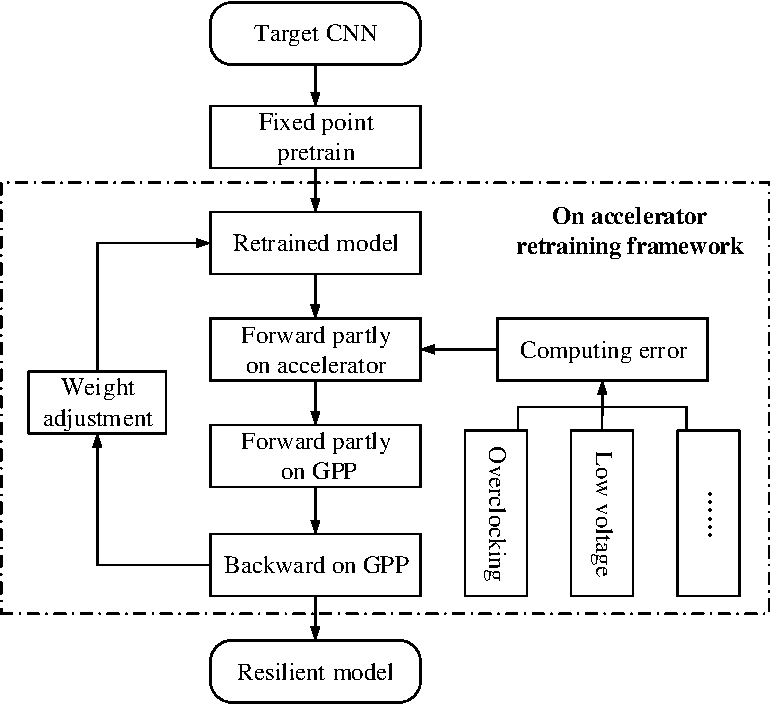
\includegraphics[width=0.85\linewidth]{on_accelerator_retrain_pocess}}
        \caption{Resilient neural network training framework}
        \label{fig:retrain}
        \vspace{-1em}
\end{figure}

\subsection{CNN accelerator abstraction and modification}
As illustrated in the above section, the forward propagation will 
mostly be executed on the CNN accelerator while 
the rest part runs on GPPs. Essentially, the framework targets at a 
heterogeneous computing architecture and frequent 
communication between the accelerator and the GPPs are expected. 
In order to fit various CNN accelerators within the same training framework,
we abstract the CNN accelerators with a high-level interface
which makes the accelerators near transparent to the training framework.
To facilitate the data communication between the forward propagation
and the rest of the training framework, we define a high-level
interface which consists of 7 functions as listed inTable \ref{tab:api}.
%Function 1 is used to launch the CNN accelerator from host. 
%Function 2 and 3 are used to transfer data between the host memory and the device memory during 
%the training. As the forward propagation on the CNN accelerators is usually fixed point 
%and the back propagation on GPPs is floating point, data type converting between fixed point 
%and floating point is required. Function 4 and 5 can be used for this purpose. 
%Function 1 to 5 are required for all the accelerators. 
%Function 6 and 7 are only used for accelerators that compute on reorganized data\cite{pipecnn_2,deepburing_12}. 
With the interface functions, general CNN accelerators can be conveniently
referenced and used in the proposed on-accelerator training framework.
\begin{table*}
	\
        \centering
        \vspace{-0.3em}
        \caption{High-level interface to integrate general CNN accelerators with Caffe}
        \label{tab:api}
        \vspace{-0.3em}
        \begin{tabular}{c|l|l}
                \toprule
                ID & Function Name & Description  \\
                \midrule
                1 & launchAccelerator() & It configures the CNN accelerator and launches it from host CPU. \\
		\midrule
                2 & dataToFPGA(weight, input, wgtDevAddr, inDevAddr) & It transfers both the input data and weight to the FPGA device memory. \\
		\midrule
		3 & dataFromFPGA(outputDevAddr, output) & \shortstack[l]{It transfers intermediate data from FPGA device memory to host memory.} \\
		\midrule
		4 & convertIntToFloat(int iData, float fData) & It converts the fixed-point point to float for back propagation processing. \\
		\midrule
		5 & convertFloatToInt(float fData,  int iData) & \shortstack[l]{It converts the floating-point input and weight to fixed point for forward processing.} \\
		\midrule
		6 & dataLayoutReorder(data, reorderedData) & \shortstack[l]{It reorders the data layout for more efficient accelerator execution.} \\
		\midrule
		7 & dataLayoutRecover(reorderedData, data) & It reorders the output data back to the default format for Caffe back propagation. \\
                \bottomrule
        \end{tabular}
        \vspace{-1em}
\end{table*}

In this work, we have the CNN accelerator implemented on Xilinx FPGAs as a case study. 
With Xilinx SDAccel, we can wrap the accelerators with OpenCL API while the accelerators 
can either be developed with OpenCL, HLS or RTL. On top of the OpenCL API, the proposed 
high-level interface can be implemented. Meanwhile, we use Caffe, a C++ based 
deep learning framework, to construct the on-accelerator training framework. With 
both parts developed with C family languages, they can be integrated conveniently. 

%In this work, we have the CNN accelerator implemented on FPGAs.
%Figure 4 depicts the implementation of the training framework on a hybrid 
%CPU-FPGA architecture. In this work, we use Xilinx KCU1500 as the FPGA board 
%and put it on a standard desktop computer. CPU is the controller and it reconfigures 
%the accelerator for a specific CNN structure. In each training iteration, CPU launches 
%the CNN accelerator to perform the forward propagation from bottom layer to top layer. 
%CPU does the backward propagation from top layer to bottom layer. Weights and the image 
%data are initially stored in host memory. It will be transferred to FPGA offchip memory 
%for forward propagation through PCI-E. Similarly, the output data will be transferred 
%from FPGA off-chip memory back to host memory after forward propagation. Because of the 
%OpenCL based API wrapper in SDAccel, the CNN accelerator’s interface can be easily 
%exposed to Caffe for referring to the forward propagation result. 

\begin{figure}
        \center{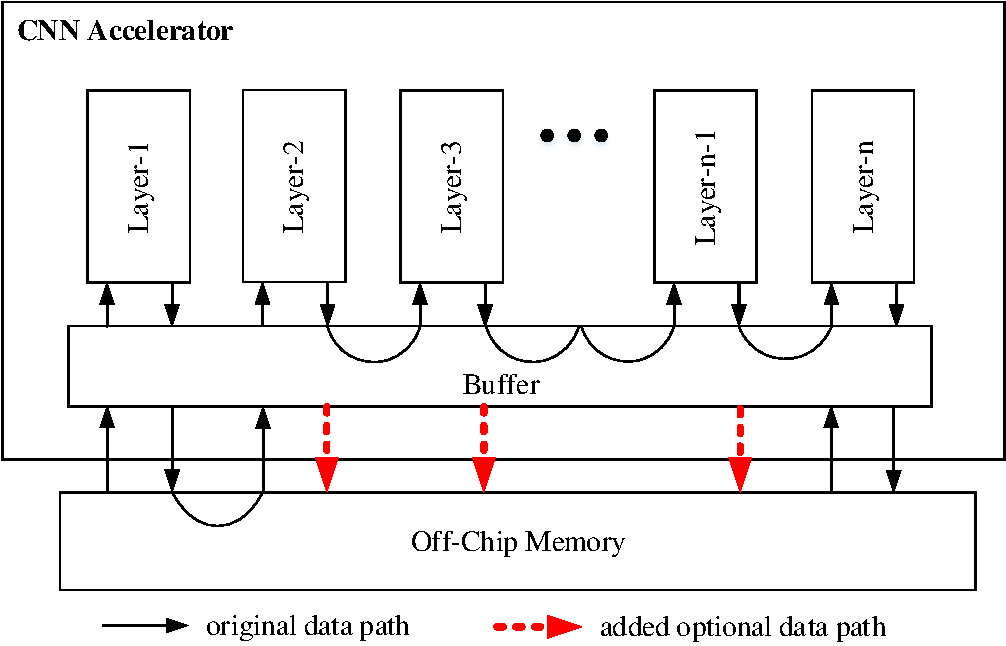
\includegraphics[width=0.85\linewidth]{change_of_accelerator}}
        \caption{Modification of the CNN accelerator data path. It essentially
ensures the feature map of each neural network layer to have an optional data path
to external memory for back propagation in training.}
        \label{fig:change_of_accelerator}
        \vspace{-1em}
\end{figure}

On top of the high-level interface, the CNN accelerator also needs 
minor modification to enable the on-accelerator training. 
The training requires the feature map of each neural 
network layer for backward propagation. However, many of the accelerators 
are intensively optimized for inference only and some of the layers' output 
are fully buffered in on-chip memory to reduce the external memory access. 
Thereby, the accelerator should provide an optional data path such that 
intermediate output data can be written to external memory at request.
As shown in Figure \ref{fig:change_of_accelerator}, the output of each layer 
will be transferred to memory using the added data path 
when the accelerator is used for training. The write back data path 
can be switched off during inference. 

\subsection{Critical neural network layer protection}
In order to improve the overall neural network resilience, we opt to 
protect the critical network layers to alleviate the resilience 
bottleneck. The protection is essentially 
to have the critical layers executed on reliable computing infrastructures 
and the exact protection method depends on the target hardware platform.
We may either schedule the critical layers to the GPPs or switch the accelerator 
to reliable mode during the execution of the critical layers.
With this approach, the overall network can tolerate 
more computing errors. 

To decide the critical layers of the neural networks, we formulate the 
critical layer selection scheme. Suppose the neural network layers include 
$N$ layers and each layer is represented as $L_i$ where $i \in {0, 1, 2, ..., N-1}$.
Then we evaluate the prediction accuracy loss of the neural network 
that have one layer protected on accelerators with computing errors.
When the $i$th layer is protected, the loss is $loss_i$.
Then the most critical layer is the layer that leads to the most 
accuracy loss i.e. $c \in \{k|loss_k = max(loss_i), i \in \{0, 1, ..., N-1\}\}$.

The above formulated approach requires large amount of evaluation of 
different layers of the neural network. Instead, we use the actual 
computing errors as the critical layer selection metric. We set an 
error threshold $T$ and assume 8bit integers are used. 
When the error equals to 0, the computing results are correct. 
When the error is larger than $T$, the results are assumed to be large errors.
When the computing results are wrong but smaller than $T$, the results are considered 
as moderate errors. The layers that include the largest portion of large errors 
are taken as the critical layers.

In addition, scheduling the neural network layers executed 
on the accelerator to GPPs has performance penalty due to the 
computing efficiency gap. As the accelerators are usually 
orders of magnitudes faster than the GPPs for neural network 
processing especially large convolution layers, we can focus on 
the last few small layers to ensure negligible performance 
loss. This constrain greatly reduces the search space
of the critical layers. 



\section{SCGRA Overlay Infrastructure} \label{sec:scgraimplement}
One key idea of QuickDough is to rely on an intermediate SCGRA overlay to improve compilation time of the high-level user application. While the exact design of this SCGRA does not affect the compilation flow, its implementation does have a significant impact on the performance of the generated gateware.
 
\subsection{SCGRA Based FPGA Accelerator}
Figure \ref{fig:scgra-accelerator} is the proposed FPGA accelerator built on top of the SCGRA overlay. The input/output data buffers and Acc Ctrl block are almost the same with those in the typical acceleration architecture \ref{fig:typical-FPGA-accelerator}, while the rest blocks are unique. 

Particularly, the kernel part of the accelerator is a synchronous 2D torus SCGRA which consists of an array of PEs. Details of the PE will be illustrated in the next section. Another major difference is that two address buffers instead of the customized logic are used as the address generator to control the on-chip buffer accessing. With the address buffers, there is no need to develop any spcific address generator when the target application changes, as we can simply replace its content together with the SCGRA configuration memory according to the scheduling result. Therefore, it reduces the chance of FPGA implementation and is beneficial to improving the design productivity. 

Finally, it is noted that input and output data buffers could accommodate more data than that used by a single SCGRA execution, so the SCGRA may iterate multiple times before it consumes all the data in input buffer or fills the output buffer. From the perspective of host processor, it is more efficient to control multiple SCGRA execution at a time instead of each SCGRA execution independently. In this case, we have a control unit called SCGRA Ctrl to make the multiple SCGRA execution transparent to the Acc Ctrl. Also sharing the data sets among multiple SCGRA execution could make best use of the limited input/output buffer. In addition, the regular SCGRA overlay tends to run at higher frequency than the data buffer controller handling the system bus protocol, and two sets of synchronous registers are added to keep the computation core and the rest of the design to running at individual clock domains.  

\begin{figure}[h]
    \center{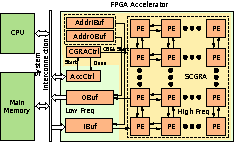
\includegraphics[width=0.8\linewidth]{scgra-accelerator}}
    \caption{SCGRA Accelerator}
    \label{fig:scgra-accelerator}
\end{figure}

\subsection{PE}
In this section, an instance of PE is presented to demonstrate the feasibility of producing high performance gateware. As shown in \figref{fig:pe}, the PE, centring an ALU block, a multiple-port data memory and an instruction memory, is highly optimized for FPGA implementation. In addition, load/store paths are implemented on the PEs that are responsible for data I/O beyond the FPGA. Addr Ctrl is used to start and reset the SCGRA execution by changing the instruction memory read address sequentially, so it has a single bit global start input signal from the SCGRA Ctrl block. 

\begin{figure}[h]
\center{\includegraphics[width=0.95\linewidth]{pe}}
\caption{PE structure}
\label{fig:pe}
\end{figure}

\subsubsection{Instruction Memory and Data Memory}
The instruction memory stores all the control words of the PE in each cycle. Since its content does not change during runtime, a ROM is used to implement this instruction memory and the content of the ROM can be loaded directly into a pre-implemented bitstream. The address of the instruction ROM is determined by the Addr Ctrl. Basically, the SCGRA execution will proceed sequentially when the start signal is valid, and it will be reset when the start signal is invalid.

Data memory stores intermediate data that can either be forwarded to the PE downstream or be sent to the ALU for calculation. For fully parallelized operation, \emph{at least} four read ports are needed -- three for the ALU and one for data forwarding. Similarly, at least two write ports are needed to store input data from upstream memory and to store the result of the ALU in the same cycle. Although a pair of true dual port memories seem to meet this port requirement, conflicts may arise if the ALU needs to read the data while the data path needs to be written. As a result, a third dual port memory is replicated in the data memory.

Note that data memory here is usually implemented using a multiple port register file in many previous CGRA work. Although register file is even more flexible in terms of parallel reading and writing, the multi-port register file size is limited due to the inefficient hardware implementation. While we have a much larger DFG for scheduling and thus larger temporary storage is required, eventually a multi-port data memory is used instead. 

\subsubsection{ALU}
At the heart of the proposed PE is an ALU designed to cover the computations in target application. \figref{fig:ALU} shows an example design that could support all the operations of our benchmark which is listed in \tabref{tab:operations}. Complex operations like MULADD/MULSUB are implemented with DSP core directly. Operations with moderate complexity like ADDADD, RSFAND etc. are divided into two stages naturally and hardware block reuse is also considered at the same time. Finally, simple operations that can be done in a single cycle can be put in either stage depending on the pipeline status. Note that MUX in data path has significant influence on timing as well, so small MUX should be inserted properly and large MUX should be avoided. Currently, we just manually create the ALU design, but it is possible to automate this step. 

\begin{figure}[h]
\center{\includegraphics[width=0.8\linewidth]{alu}}
\caption{ALU Example}
\label{fig:ALU}
\end{figure} 

\begin{table}[h]
\caption{Operation Set Implemented in ALU}
\label{tab:operations}
\centering
\begin{tabular}{|p{1.5cm}|p{1.5cm}|p{4cm}|}
\hline
Type & Opcode & Expression \\

\hline
MULADD & 0001 & {dst = src0 $\times$ src1 + src2} \\

\hline
MULSUB & 0010 & {dst = src0 $\times$ src1 - src2} \\

\hline
ADDADD & 0011 & {dst = src0 + src1 + src2} \\

\hline
ADDSUB & 0100 & {dst = src0 + src1 - src2} \\

\hline
SUBSUB & 0101 & {dst = src0 - src1 - src2} \\

\hline 
PHI & 0110 & {dst = src0 ? src1 : src2} \\

\hline
RSFAND & 0111 & {dst = (src0 $\gg$ src1) \& src2} \\

\hline
LSFADD & 1000 & {dst = (src0 $\ll$ src1) + src2} \\

\hline
ABS & 1001 & {dst = abs(src0)} \\

\hline
GT & 1010 & {dst = (src0 $>$ src1) ? 1 : 0} \\

\hline
LET & 1011 & {dst = (src0 $\leq$ src1) ? 1 : 0} \\

\hline
ANDAND & 1100 & {dst = src0 \& src1 \& src2} \\

\hline
\end{tabular}
\end{table}

\subsection{Load/Store Interface}
For the PEs that also serve as IO interface to the SCGRA, they have additional load path and store path as shown in \ref{fig:pe}. Load path and the SCGRA neighboring input share a single data memory write port, and an additional pipeline stage is added to keep the balance of the pipeline. Store path has an additional data MUX as well, but it doesn't have significant influence on the rest of the design. 


\section{Application Compilation} \label{sec:scgracompile}

The QuickDough compilation process consists of four main inter-related steps as illustrated in \figref{fig:scgra-compile}.  In the first step, compute kernels of the application are extracted and transformed into their corresponding dataflow graphs (DFGs).  Then, the corresponding overlay is created either by reusing an existing implementation or by synthesizing a new application-specific overlay based on an architectural template.
In the third step, the DFGs and hyperblocks are scheduled to the generated overlay using an operation scheduler.
Finally, the operation schedule is extracted and the corresponding configuration words are integrated into the configuration bitstream of the overlay.  In our current implementation, the \texttt{data2mem} tool from Xilinx is used for this purpose.

\begin{figure}
\center{\includegraphics[width=0.8\linewidth]{scgra-compile}}
\caption{SCGRA compilation with customized overlay and specified compute kernel.}
\label{fig:scgra-compile}
\end{figure}

%As the simulation performance of the DFG and block can be acquired from the scheduling, with the pre-built SCGRA implementation frequency and the communication efficiency of the compute system, we can obtain even accurate performance of the compute kernel and can further check whether the performance goal is met. If the design goal is not met, we can go back to the block and DFG generation stage altering the design options such as loop unrolling factor. Repeat these steps until the design goal is achieved.

Among them, the physical implementation of the overlay is obviously the most time consuming.
To ensure a rapid compilation experience, the user may want to generate a new overlay architecture only as needed, perhaps on a per-application domain basis.  It is important to note, however, that the application remains functionally correct even when it is executed on a suboptimal overlay configuration.
The user may therefore take advantage of the fast compilation to the overlay during initial development phases that demand rapid debug-edit-cycles.
Once the function of the accelerator is confirmed, the user may proceed with customizing the overlay architecture for performance sake.


\subsection{DFG Generation \& Grouping}
The main input to the QuickDough framework for acceleration are compute intensive kernels extracted from the user applications.  The first step of the compilation process is therefore to extract dataflow graphs (DFGs) from these kernels that are often expressed as inner loop bodies.
Depending on its structure, this loop may further be unrolled multiple times to increase the amount of operation parallelism in the generated DFG.  During run time, the generated DFG will be executed repeatedly until the end of the original loop.  \figref{fig:blocking-and-dfg-gen} illustrate this process.

\begin{figure}
\center{\includegraphics[width=0.8\linewidth]{dfg-gen}}
\caption{Relation between compute kernel, group and DFG. Data transmission between FPGA and host CPU is
performed for each group execution.}
\label{fig:blocking-and-dfg-gen}
\end{figure}

In addition to unrolling the innermost loops, the QuickDough framework also allows users to balance computation and communication by batching data transfers for multiple executions of the same DFG into groups as shown in \figref{fig:blocking-and-dfg-gen}.
Specifically, after the loop is unrolled $U$ times, $G$ of them are grouped together for each data transfer.
During each data transfer, input data for all $G$ iterations will be sent to the accelerators.
They are stored in the on-chip buffer so they can be accessed by the processing array within a single cycle.

While grouping data transfers helps amortize the communication cost between CPU and the accelerator, it also imposes additional requirement for on-chip memory to serve as buffer for the extra data transferred.
As a result, the unrolling factor $U$ and grouping factor $G$ has to be co-optimized to balance performance and on-chip resource utilization.
For instance, increasing $U$ leads to a larger DFG to be executed in the QuickDough overlay, which may be benefited from a larger processing array.  However, the increased processing array limits the amount of on-chip buffer available for data and address buffer.  As a result, the amount of DFG grouping $G$ is limited and may lead to higher performance penalty due to communication.

A fully automated customization framework that optimizes such parameters is beyond the scope of this work.  However, different unrolling and grouping factors in the benchmark will be explored in \secref{sec:experiments}.



%The communication between the processor and the accelerator is costly. When the data size of a DFG is small, data transmission for each DFG execution may compromise all the benefits of the accelerator. To solve this problem, we have the accelerator to repeat the DFG execution multiple times and combine them as a block. Data transmission is performed with the granularity of a block instead of a DFG which helps to amortize the initial communication overhead especially for the DMA transmission. \figref{fig:blocking-and-dfg-gen} shows the relation among the compute kernel, block and DFG using a simple example. 


%Since the SCGRA employs lock-step execution and the input/output data for each block execution must also be fully buffered, the block size is mainly limited by the data buffer size. 


%Given the block size, we need further to decide the loop unrolling factor such that the unrolled part can be transformed to DFG which can be executed on the SCGRA. Usually, the unrolling factor is limited by the instruction memory and data memory. 

%In addition, we have straightforward address buffers which store all the on chip buffer accessing addresses of the whole block execution. Although it is already set to be twice larger than the data buffer, it still overflows easily and becomes another major limitation of both the block size and the unrolling factor. Finally, the compute kernel depends on the repeating of the block execution and the block execution depends on the repeating of the DFG execution. As a result, the loop count must be fully divided by the block size and the block size must also be fully divided by the unrolling factor. This can be another unrolling and blocking limitation as well. 


\subsection{Overlay Generation}
The QuickDough overlay is a highly regular processing array that can be generated easily according to a template.
The overlay may be customized in many aspects, including the type of operation supported by each processing element (PE), the processing array size, its topology, as well as the number and capacity of the data buffers.
For sake of rapid compilation, presynthesized overlay may be used.
To improve performance, or to customize the type of operation for a new application, the user may opt to synthesize a new overlay design that may be reused subsequently.
Similar to the case of DFG generation, the discussion of a fully automated optimization framework that optimizes the overlay design to the application is beyond the scope of this work.
Instead, we examine multiple overlay configurations in the benchmark session to experiment tradeoffs that are involved.

\subsection{Operation Scheduling}
Once the overlay architecture is determined, the operations from the user DFG are scheduled to execute on the reconfigurable array.
Since the processing elements in the QuickDough overlay execute in lock steps with deterministic latencies, a classical list scheduling algorithm \cite{schutten1996list} was adopted.
The challenge in this scheduler is that data communication among the processing elements must be carried out via multi-hop routing in the array.
As a result, while it is desirable to schedule data producers and consumers in nearby processing elements to minimize communication latencies, it is also necessary to utilize as much parallel processing power as possible for sake of load balancing.
Building on top of our previous work presented in \cite{colinheart}, a scheduling metric considering both load balancing and communication cost was adopted in our current implementation.

 \begin{algorithm}
 \small
 \caption{The QuickDough scheduling algorithm.}
 \label{alg:scheduling}
 \begin{algorithmic}
 \PROCEDURE{ListScheduling}
 \STATE Initialize the operation ready list $L$
 \WHILE {$L$ is not empty}
 \STATE select a PE $p$
 \STATE select an operation $l$
 \STATE OPScheduling($p$, $l$)
 \STATE Update $L$
 \ENDWHILE
 \ENDPROCEDURE
 \STATE
 \PROCEDURE {OPScheduling($p$,$l$)}
 \FORALL {predecessor operations $s$ of $l$}
 \STATE Find nearest PE $q$ that has a copy of operation $s$
 \STATE Find shortest routing path from PE $q$ to PE $p$
 \STATE Move operation $s$ from PE $q$ to PE $p$ along the path
 \ENDFOR
 \STATE Do operation $l$ on PE $p$
 \ENDPROCEDURE

 \end{algorithmic}
 \end{algorithm}

\algref{alg:scheduling} briefly illustrates the scheduling algorithm implemented in QuickDough. Initially, an operation ready list is created to represent all operations that are ready to be scheduled.
The next step is to select a PE from the SCGRA and an operation from the ready list using a combined communication and load balance metric.
When both the PE and the operation to be scheduled are determined, the \code{OPScheduling} procedure starts. It determines an optimized routing path, moves the source operands to the selected PE along the path, and schedules the selected operation to execute accordingly.
After this step, the ready list is updated as the latest scheduling may produce more ready operations.
This \code{OPScheduling} procedure is repeated until the ready list is empty.
Finally, given the operation schedule, the corresponding control words for each PE and the IO buffer accessing sequence will be produced.
These control words will subsequently be used for bitstream generation in the following compilation step.

\subsection{Bitstream Integration}
The final step of the compilation is to generate the instructions for each PE and the address sequences for the I/O buffers according to the scheduler's result, which will subsequently be incorporated into the configuration bitstream of the overlay produced from previous steps.
By design, our overlay does not have any mechanism to load instruction streams from external memory.
Instead, we take advantage of the reconfigurability of SRAM based FPGAs and store the cycle-by-cycle configuration words using on-chip ROMs. The content of the ROMs are embedded in the bitstream and the \code{data2mem} tool from Xilinx \cite{data2mem} is used to update the ROM content of the pre-built bitstream directly. To complete the bitstream integration, \code{BMM} file that describes the organization and placements of the ROMs in the overlay is extracted from \code{XDL} file corresponding to the overlay implementation \cite{beckhoff2011xilinx}.
This bitstream integration process costs only a few seconds of the compilation time.




\section{Experiments and results} \label{sec:result}
The experiments mainly include two parts. In the first part, we 
analyze the implementations of the SCGRA overlay based FPGA accelerators with 
different configurations to demonstrate the regularity of the 
SCGRA overlay based FPGA accelerators. In the second part, we benchmark the 
efficiency and quality of the proposed customization framework.

\subsection{Experiment Setup}
All the run time was obtained from a computer with Intel(R) Core(TM) 
i5-3230M CPU and 8GB RAM. Zedboard which has an ARM processor and 
an FPGA was used as the hybrid computation system. Vivado 2013.3 was 
used for the HLS based design and PlanAhead 14.7 was used for the SCGRA overlay based 
design. 

The overlay implementations on Zedboard typically run at 200MHz and we 
assume the implementation frequency can be scalable to all the 
different overlay configurations. The power consumption used in this work was 
obtained from XPower which is part of the Xilinx design suite.

\subsection{SCGRA Overlay Implementation Analysis}
In order to analyze the overhead and power of the SCGRA overlay 
based FPGA accelerators, we had three groups of accelerators 
(SCGRA1, SCGRA2, SCGRA3) implemented on Zedboard. The configurations 
are detailed in \tabref{tab:config}. Despite of the diverse 
configurations, all the implementations could meet 200MHz 
timing constrain. With this timing constrain, 
hardware overhead and power consumption are analyzed in the 
following sub sections.
\begin{table}[tb]
    \small
    \centering
    \caption{SCGRA Based FPGA Accelerator Configuration \label{tab:config}}{
        \begin{tabular}{c|c|c|c|c|c}
            \hline
            Group & Size & \tabincell{c}{Inst. \\ Rom} & 
            \tabincell{c}{Data \\ Mem} & \tabincell{c}{IBuf \\ /OBuf} & 
            \tabincell{c}{Addr \\Buf} \\ \hline

            SCGRA1 & \tabincell{l}{2x2, 3x2, \\ 3x3, 4x3, \\ 4x4, 5x4} & 
            1kx72 & 256x32 & 2kx32 & 4kx16\\ \hline

            SCGRA2 & \tabincell{l}{2x2, 3x2, \\ 3x3, 4x3, \\4x4} & 
            2kx72 & 256x32 & 2kx32 & 4kx16\\ \hline

            SCGRA3 & \tabincell{l}{2x2, \\ 3x2, \\ 3x3 } &  
            4kx72 & 256x32 & 2kx32 & 4kx16\\ \hline
        \end{tabular}
    }
\end{table}

\subsubsection{Hardware Overhead}
\figref{fig:SCGRA-Overhead} shows the relation between 
the four types of hardware resource overhead and SCGRA 
overlay size. It can be found that FF, LUT and DSP overhead 
do not change much with the memory configurations and they 
present good linearity to the overlay size, thus they can be 
estimated with linear models. BRAM overhead depends 
on both the overlay size and the memory configurations, 
and single variable linear model will not work for the estimation.
Fortunately, it can be calculated precisely with the memory 
configurations. 

\begin{figure}[tb]
    \subfloat[\label{fig:FF-Overhead}]{%
      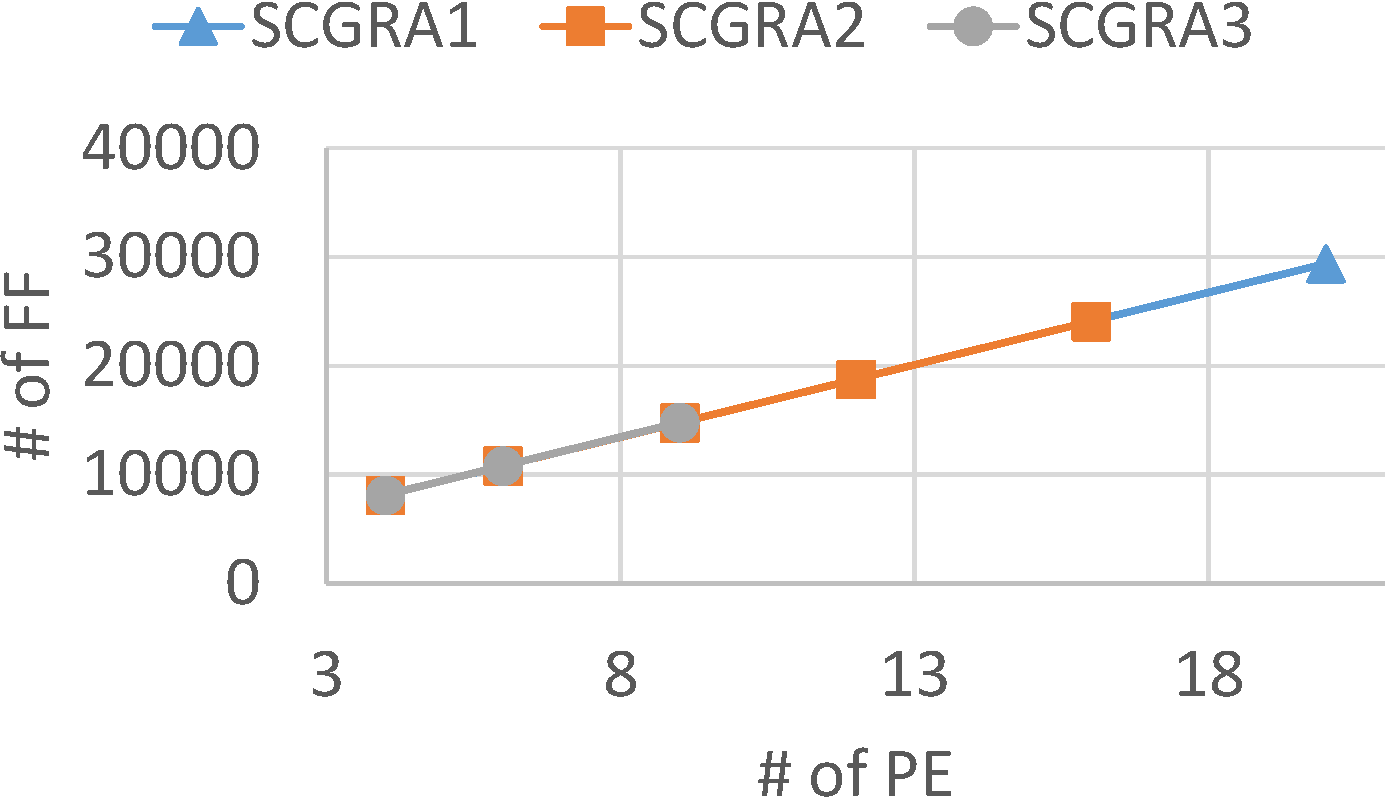
\includegraphics[width=0.22\textwidth]{FF-Overhead}
    }
    \subfloat[\label{fig:LUT-Overhead}]{%
      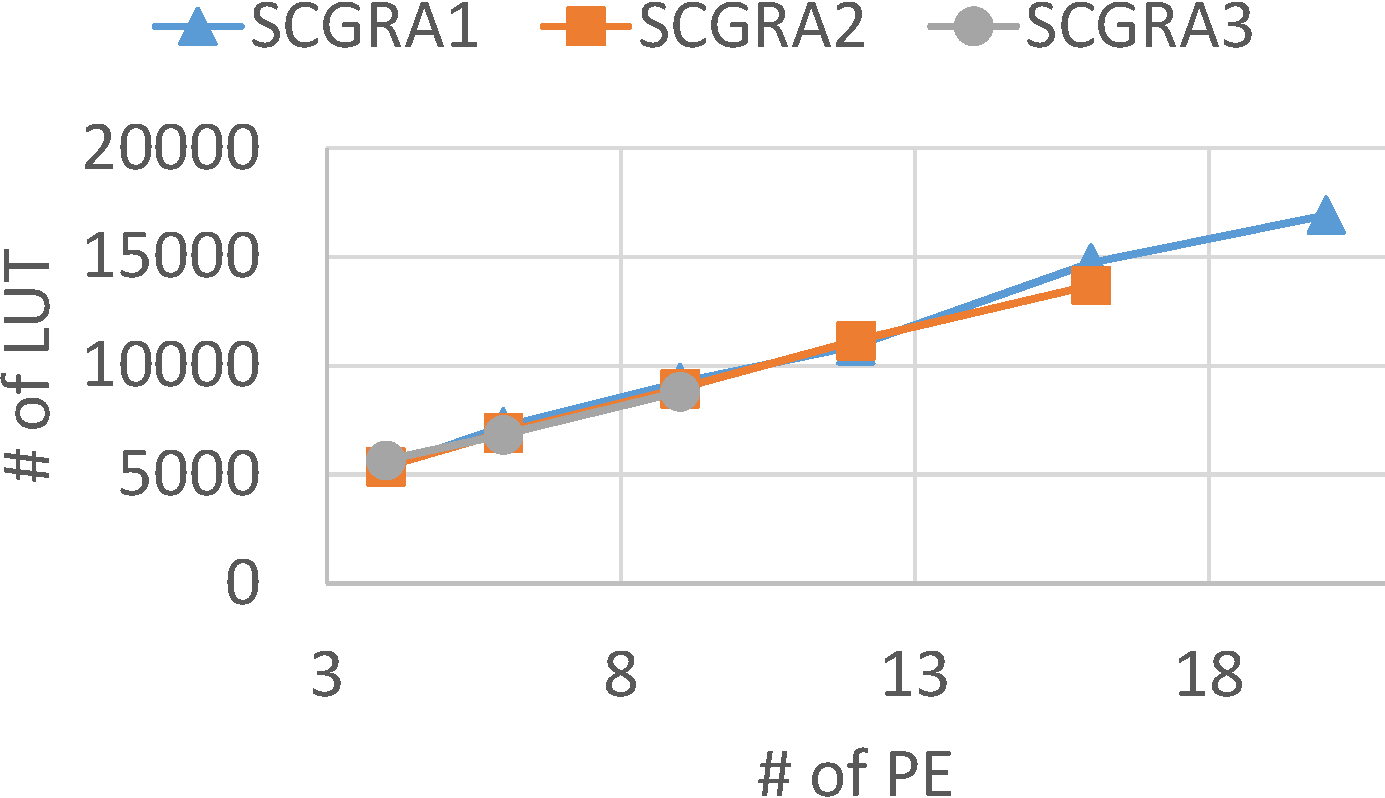
\includegraphics[width=0.22\textwidth]{LUT-Overhead}
    }
    \hfill
    \subfloat[\label{fig:DSP-Overhead}]{%
      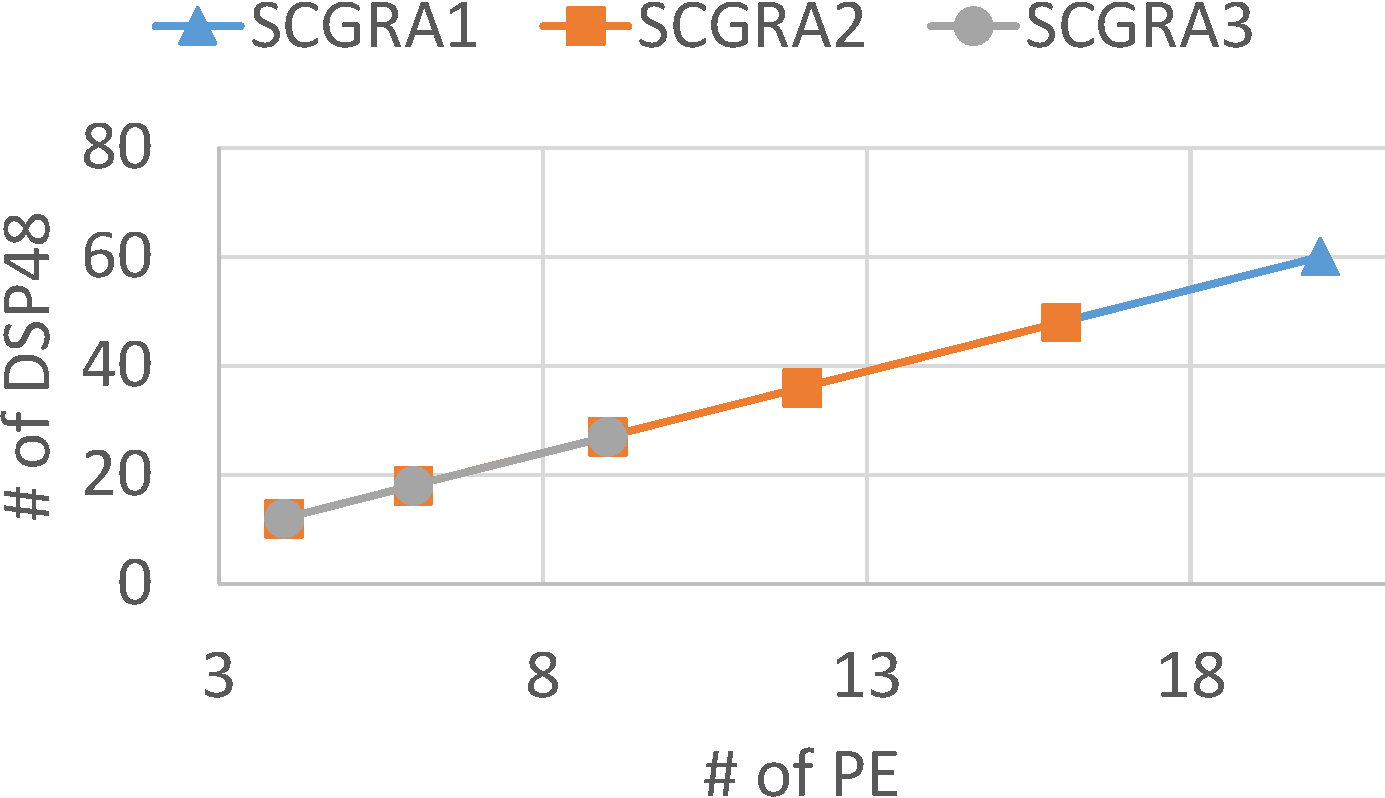
\includegraphics[width=0.22\textwidth]{DSP-Overhead}
    }
    \subfloat[\label{fig:BRAM-Overhead}]{%
      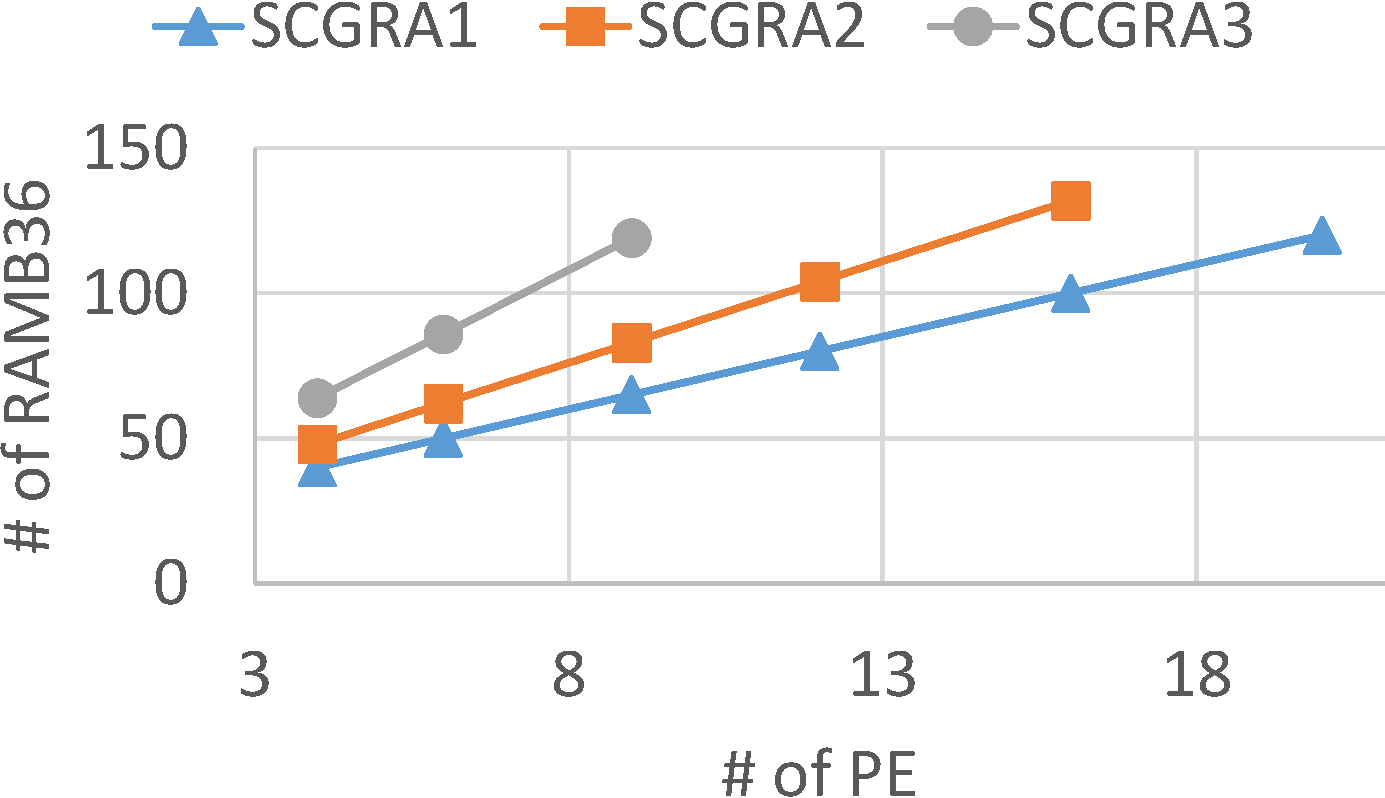
\includegraphics[width=0.22\textwidth]{BRAM-Overhead}
    }
    \caption{Relation between the accelerator overhead and overlay size, 
    (a) FF overhead, (b) LUT overhead, (c)DSP overhead, (d)BRAM overhead}
    \label{fig:SCGRA-Overhead}
\end{figure}


\subsubsection{Power Consumption}
According to the power decomposition in Xpower, the power consumption 
of an FPGA design includes signal power, clock power, BRAM power and so on. 
To simplify the power model of the SCGRA overlay based FPGA accelerator, 
we divide the power consumption into BRAM power and base system 
power which essentially includes the power consumption of the rest part of the system. 
As shown in \figref{fig:SCGRA-Power}, the base system power exhibits good linearity 
over the SCGRA overlay size while the BRAM power is near linear to 
the BRAM overhead. Therefore, both of them can be easily estimated with linear models. 

\begin{figure}[tb]
    \subfloat[\label{fig:Base-Power}]{%
      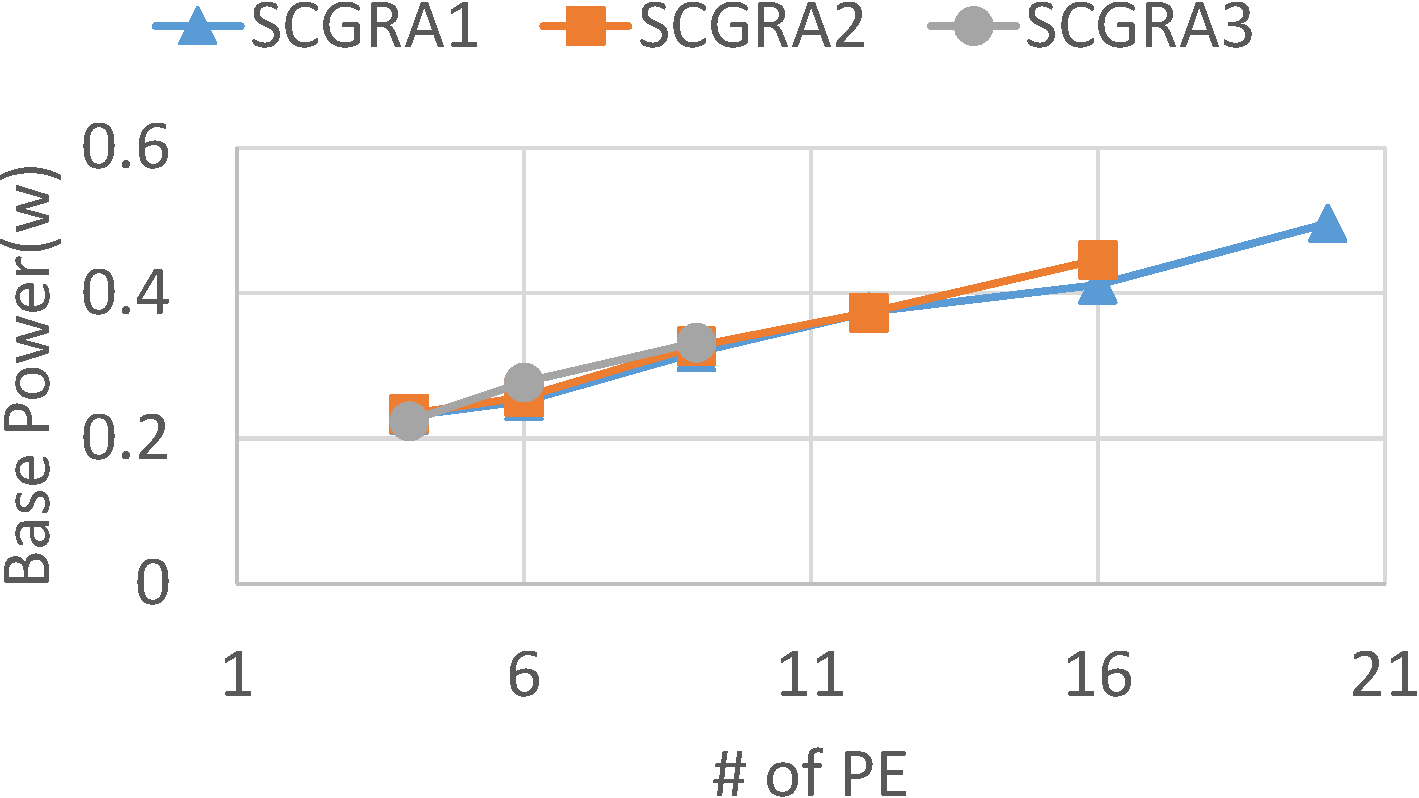
\includegraphics[width=0.22\textwidth]{Base-Power}
    }
    \subfloat[\label{fig:BRAM-Power}]{%
      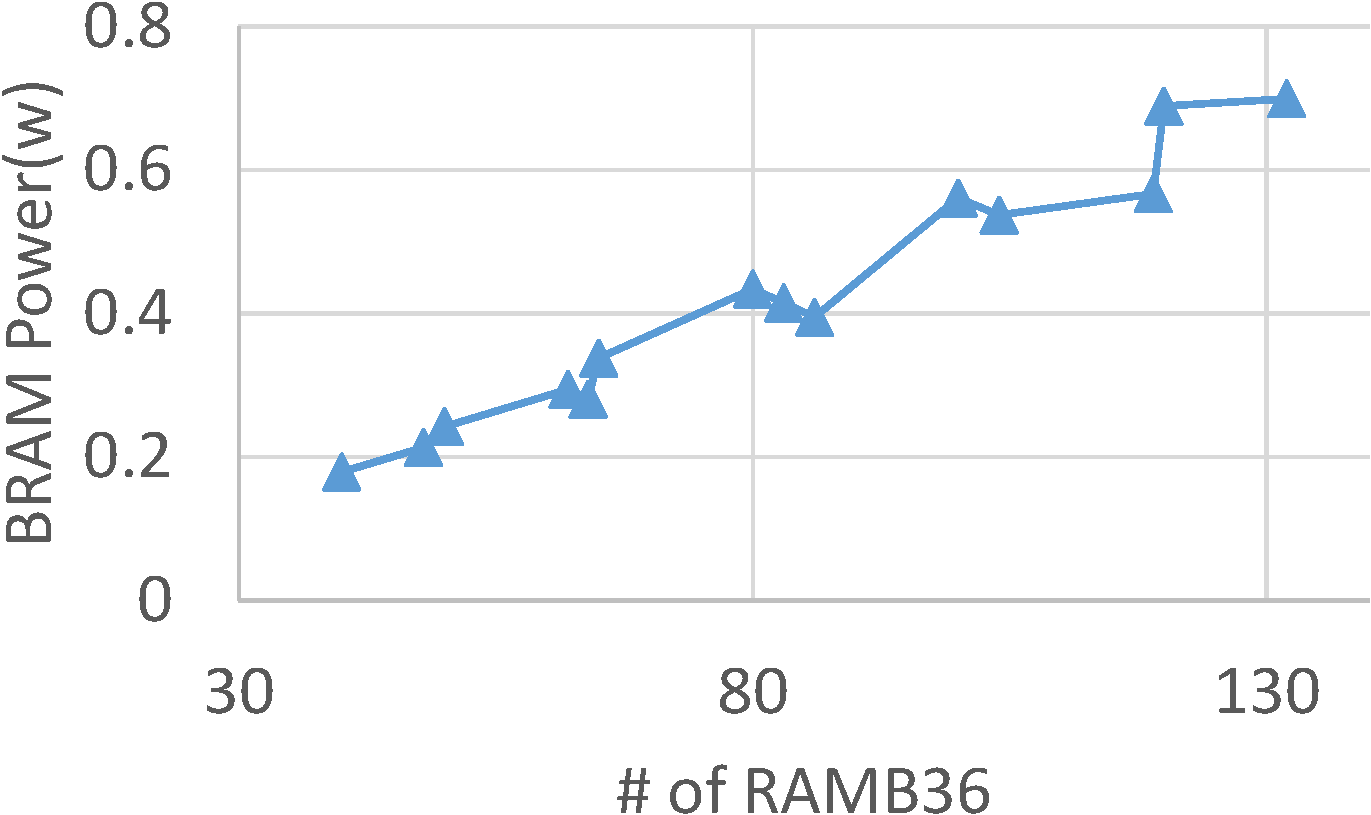
\includegraphics[width=0.22\textwidth]{BRAM-Power}
    }
    \caption{Power consumption of the SCGRA overlay based FPGA accelerator, 
    (a) Base system power including DSP power, clock power, etc., (b) BRAM power}
    \label{fig:SCGRA-Power}
\end{figure}

\subsection{Proposed Design Framework Evaluation}
In this work, we take four applications including Matrix Multiplication (MM), 
FIR, Kmean(KM) and Sobel Edge Detector (SE) as our benchmark. The 
configurations of the benchmark are detailed in \tabref{tab:benchmark-config}. 
In order to evaluate the efficiency and quality of the proposed design 
framework, we have the benchmark implemented using both the proposed 
two-step customization (TS) method and an exhaustive search (ES) 
method. Then we compared the Pareto-optimal curves acquired 
using both methods. In addition, we also have the benchmark 
implemented using Vivado HLS with moderate manual optimization 
and compare the implementations with our customized implementations. 

\begin{table}[tb]
    \small
    \centering
    \caption{Benchmark Configurations \label{tab:benchmark-config}}{
        \begin{tabular}{l|l|l}
            \hline
            Benchmark & Parameters & Loop Structure \\ \hline
            MM & Matrix Size(128) & $128 \times 128 \times 128$ \\ \hline
            FIR & \tabincell{l}{\# of Input (1024) \\ \# of Taps+1 (64)} & $1024 \times 64$ \\ \hline
            SE & \tabincell{l}{ \# of Vertical Pixels (128) \\ \# of Horizontal Pixels (8)} & $128 \times 8 \times 3 \times 3$ \\ \hline 
            KM & \tabincell{l}{\# of Nodes(1024) \\ \# of Centroids(4) \\ \# of Dimensions(2)} & $1024 \times 4 \times 2$ \\ \hline  
        \end{tabular}
    }
\end{table}

\subsubsection{Customization Methods Comparison}
\figref{fig:DSE-Time} shows the DSE time of both the TS DSE and ES DSE. 
The proposed TS DSE is around 100x faster than the ES DSE on 
average. In particular, it can be found that ES DSE can be 
extremely slow on MM which has three levels of loop with relatively large 
loop count and thus larger design space. Though TS DSE also needs 
longer time to complete the DSE of MM, it can skip most 
of the unfeasible configurations and the runtime is 
less sensitive to the size of the design space. 

\begin{figure}[tb]
    \centering
    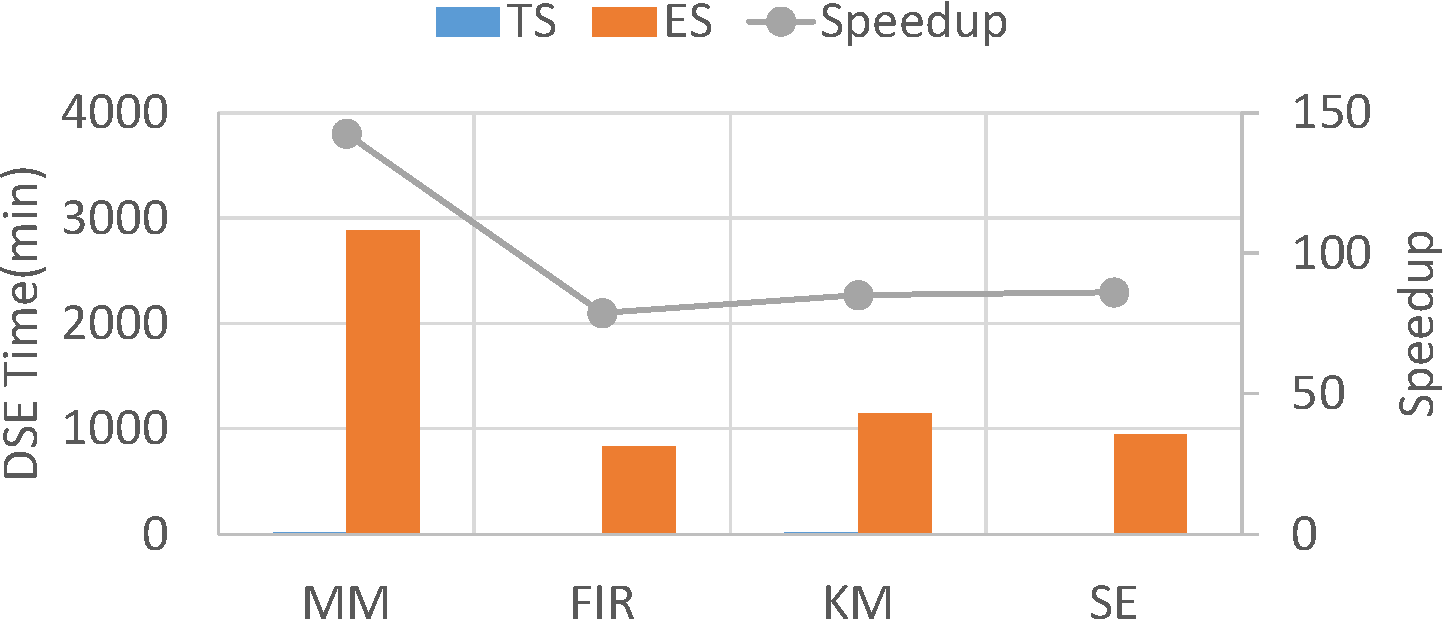
\includegraphics[width=0.35\textwidth]{DSE-Time}
    \caption{DSE time of the benchmark using both TS and ES}
    \label{fig:DSE-Time}
\end{figure}

%\begin{table}[tb]
%    \small
%    \centering
%    \caption{Time Cost for RA DSE and ES DSE\label{tab:dsetime}}{
%        \begin{tabular}{l|l|l|l|l}
%            \hline
%            Benchmark & MM & FIR & KM & SE \\ \hline
%            RA DSE (min) & 20.2 & 10.6 & 13.4 & 11.4\\ \hline
%            ES DSE (min) & 2880.6 & 835.2 & 1140.5 & 946.2\\ \hline
%            Speedup & 142.6 & 78.8 & 85.1 & 86.2 \\ \hline
%        \end{tabular}
%    }
%\end{table}

In order to demonstrate the quality of proposed framework, we presented the 
Pareto-optimal curves acquired from both DSE methods as shown in \figref{fig:DSE}. 
It is clear that the Pareto-optimal curves obtained via the two DSE methods are quite 
close. Since TS DSE may prune the design options that involve a larger 
overlay size and better performance according to the sub DSE metric, 
the Pareto-optimal curves may deviate slightly at the higher performance area. 
Fortunately, this can be improved by lowering user defined metric $\epsilon$ 
while affording longer DSE time. When we customize the design for minimum energy 
consumption, TS DSE can achieve the optimal design in all the benchmarks. 

\begin{figure}[tb]
	\subfloat[MM]{%
		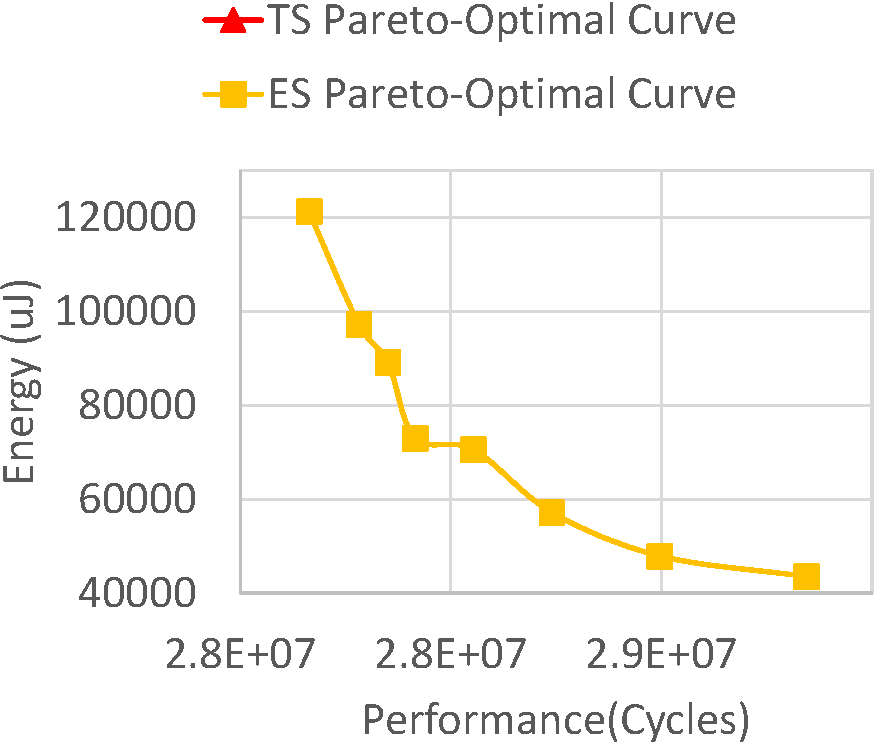
\includegraphics[width=0.22\textwidth]{mm-energy-performance}
	}
	\subfloat[FIR]{%
		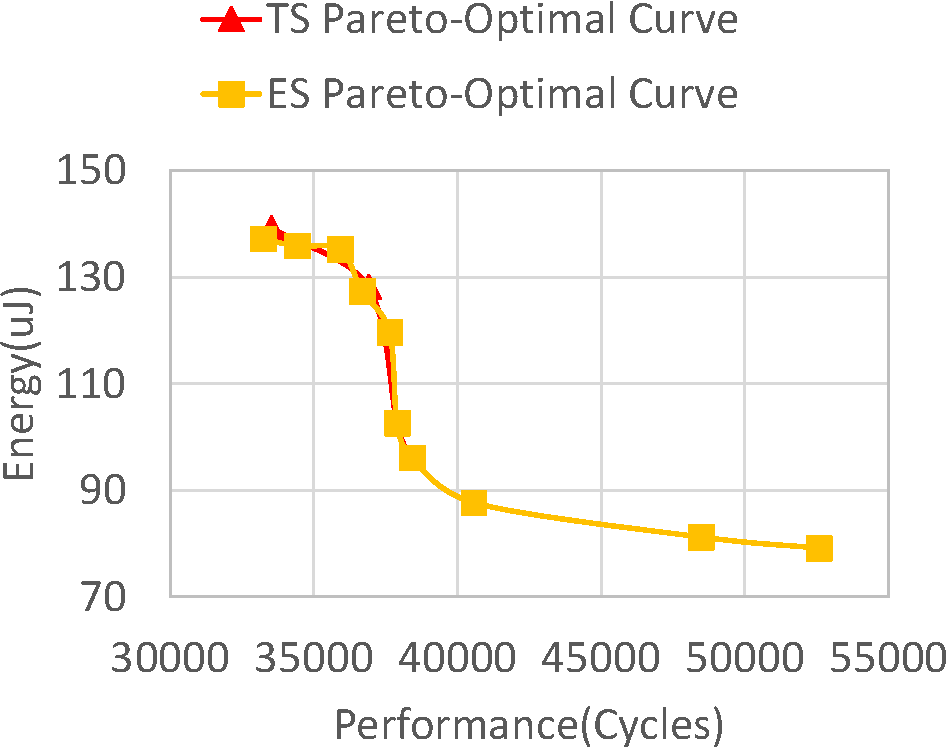
\includegraphics[width=0.22\textwidth]{fir-energy-performance}
	}
    \hfill
	\subfloat[SE]{%
		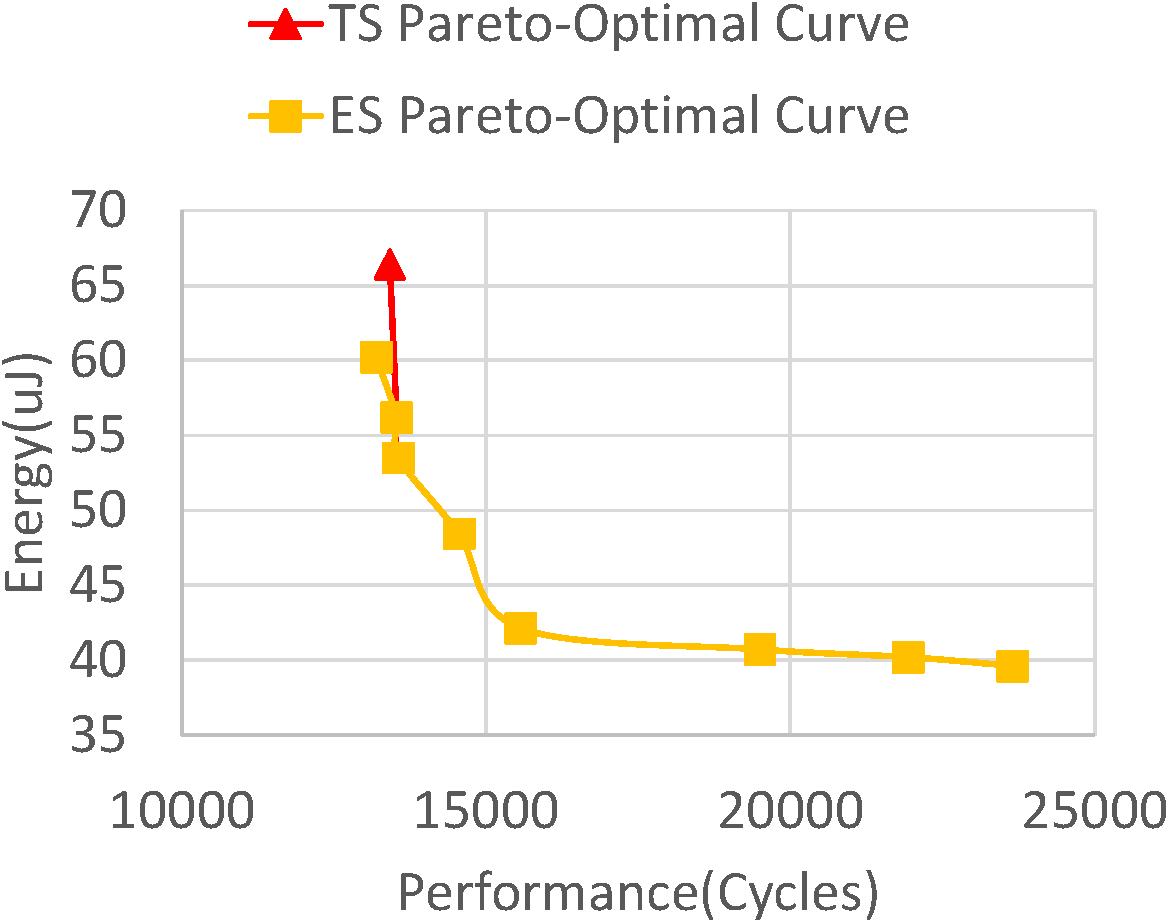
\includegraphics[width=0.22\textwidth]{se-energy-performance}
	}
	\subfloat[KM]{%
		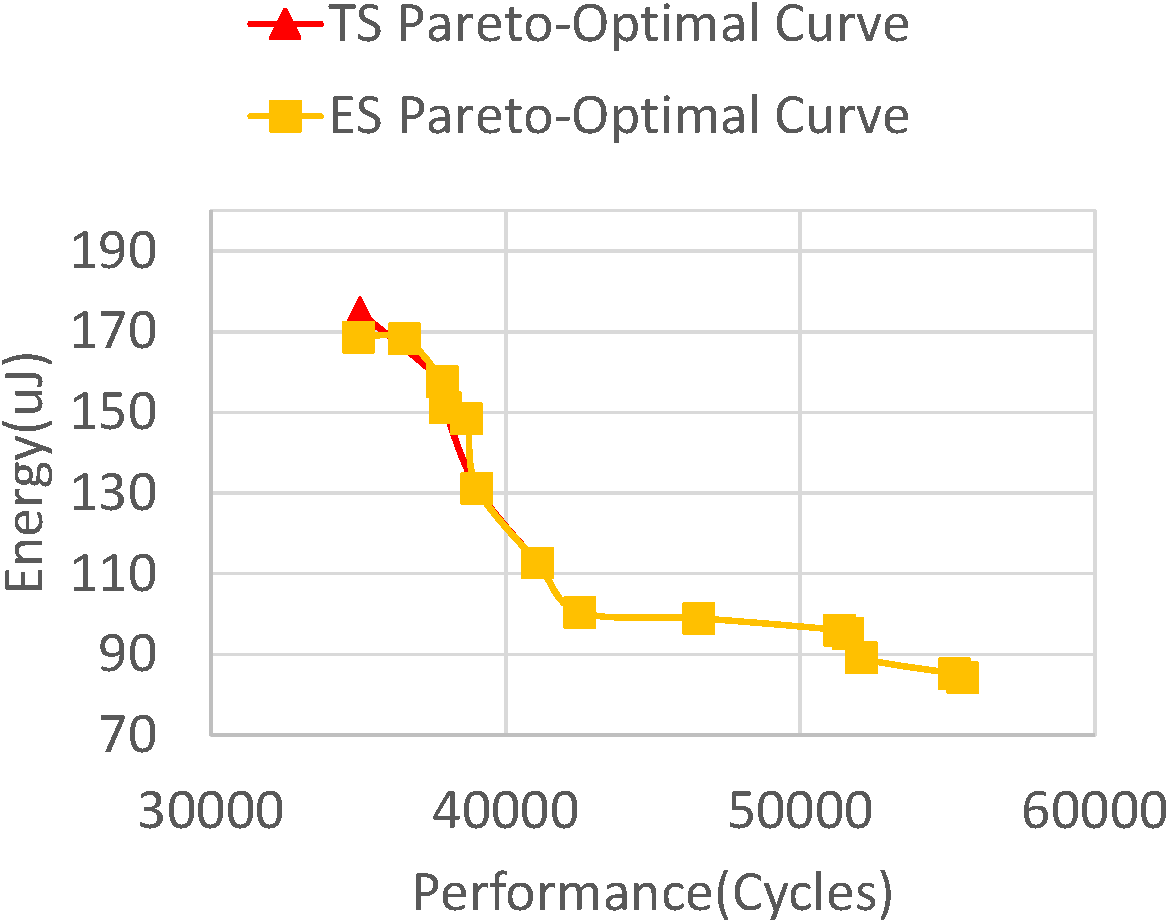
\includegraphics[width=0.22\textwidth]{km-energy-performance}
	}
    \caption{Performance-Energy Pareto-optimal curve}
	\label{fig:DSE}
\end{figure}

\subsubsection{Design Tools Comparison}
The proposed design framework will not be as useful if the performance of the 
generated system is not at least on par with similar systems created with 
conventional high-level synthesis tools. For that, we further implemented the 
benchmarks using Vivado HLS with moderate effort. The loops in the benchmark will 
be unrolled as much as possible and the input/output buffers are set as large 
as possible. Then the accelerators generated using both tools are compared. 
Since similar comparison has already been done in previous work \cite{scgra-orig}, 
we just brief the performance comparison for a quick reference.

\begin{figure}[tb]
	\subfloat[MM]{%
		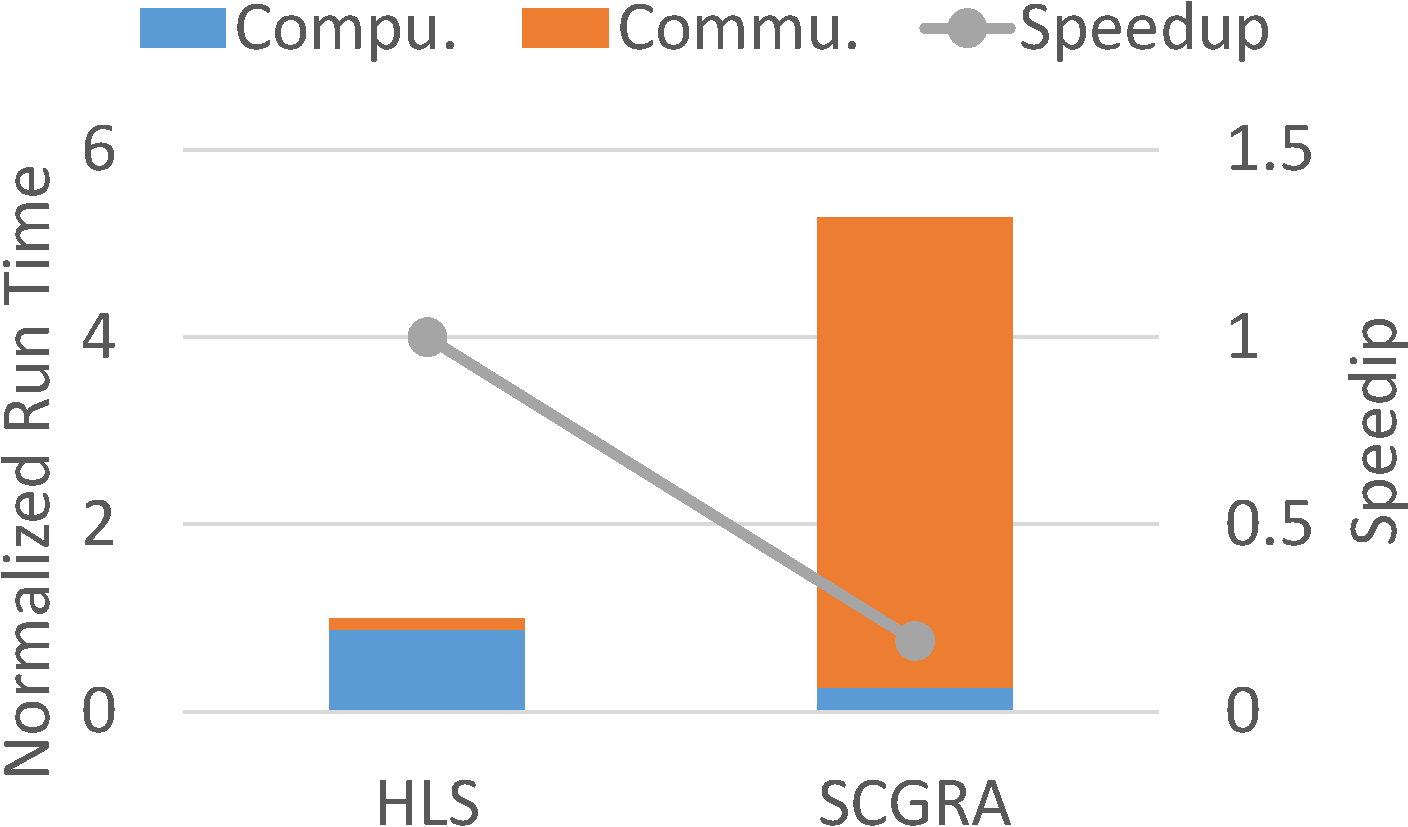
\includegraphics[width=0.22\textwidth]{mm-hls-cp}
	}
	\subfloat[FIR]{%
		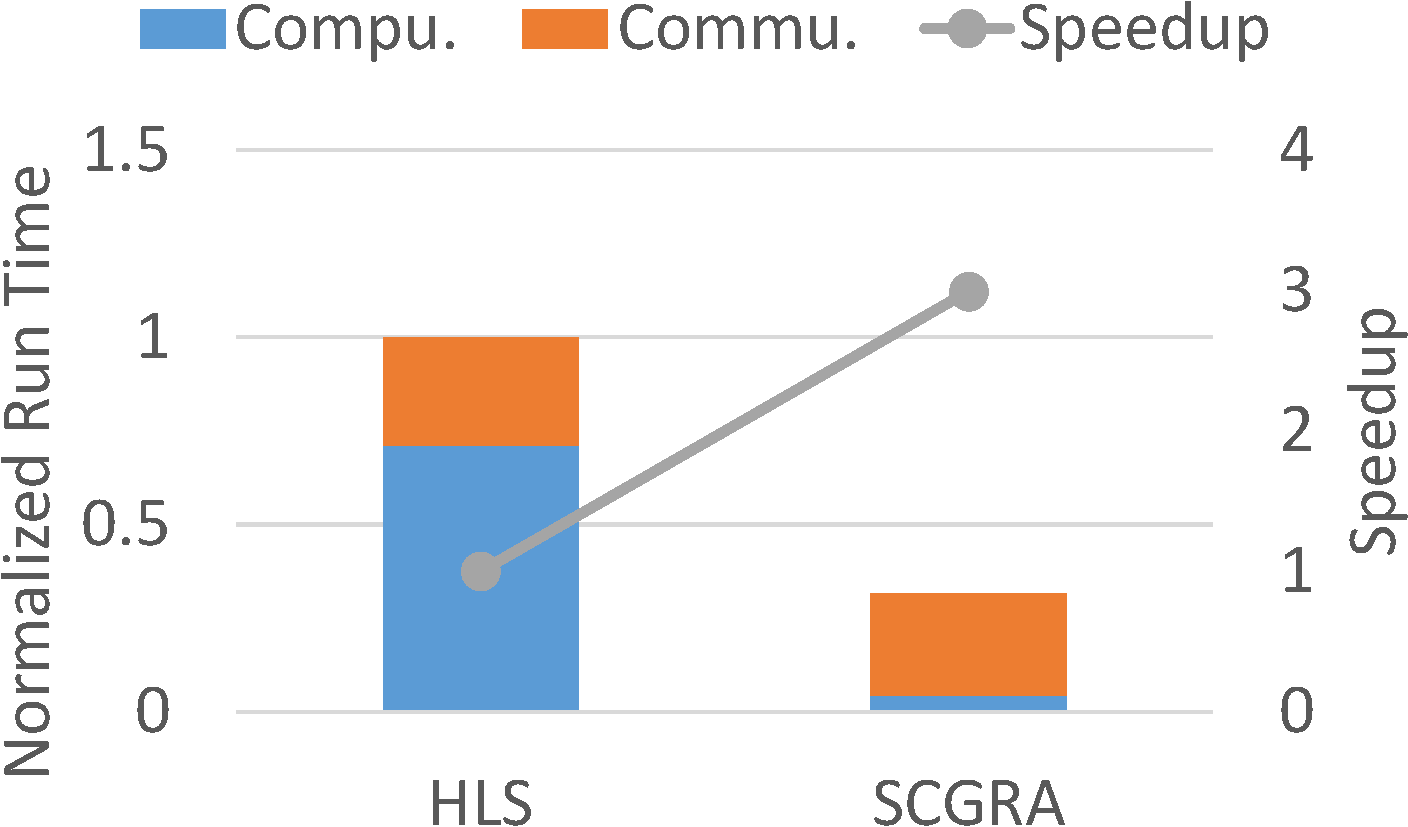
\includegraphics[width=0.22\textwidth]{fir-hls-cp}
	}
    \hfill
	\subfloat[SE]{%
		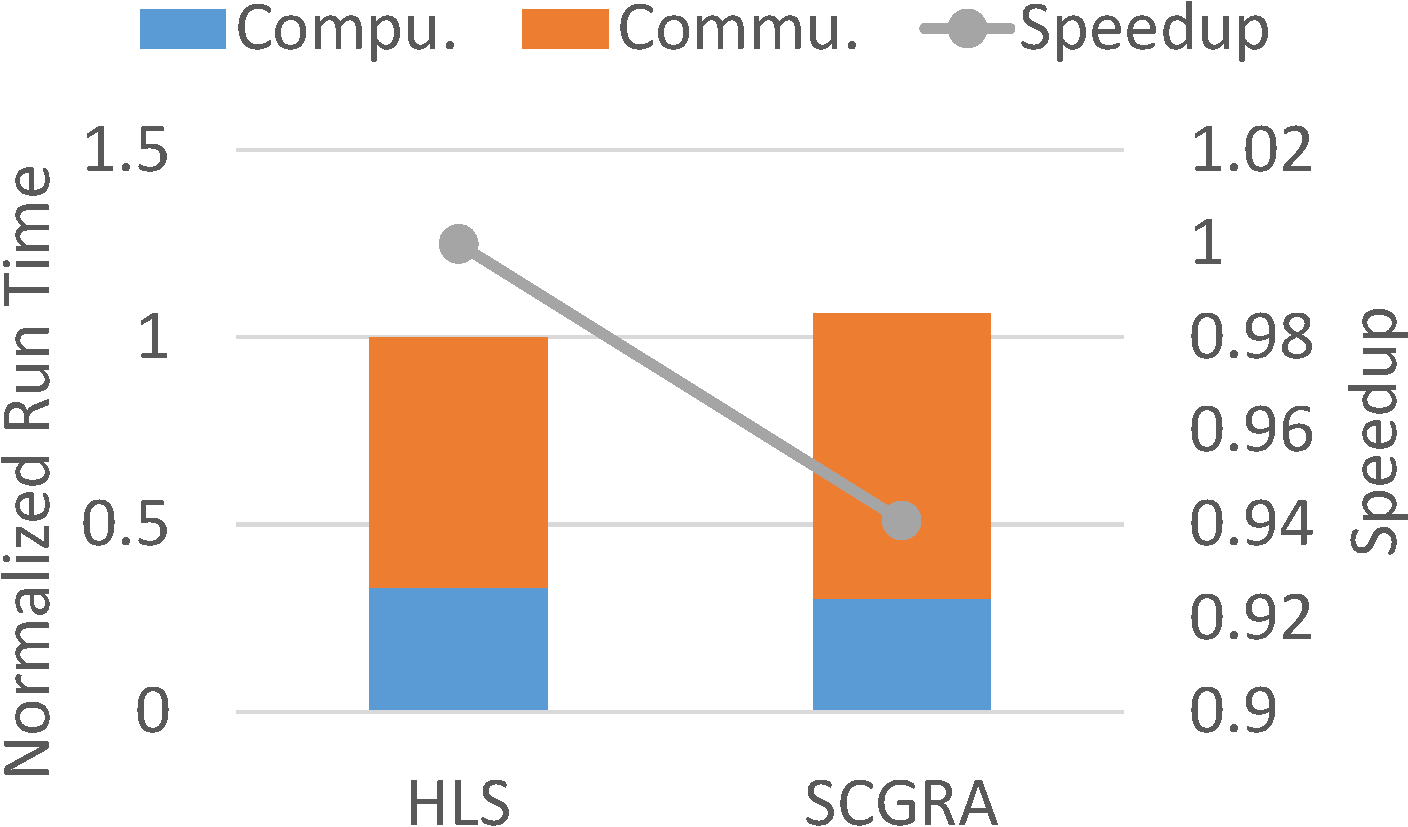
\includegraphics[width=0.22\textwidth]{se-hls-cp}
	}
	\subfloat[KM]{%
		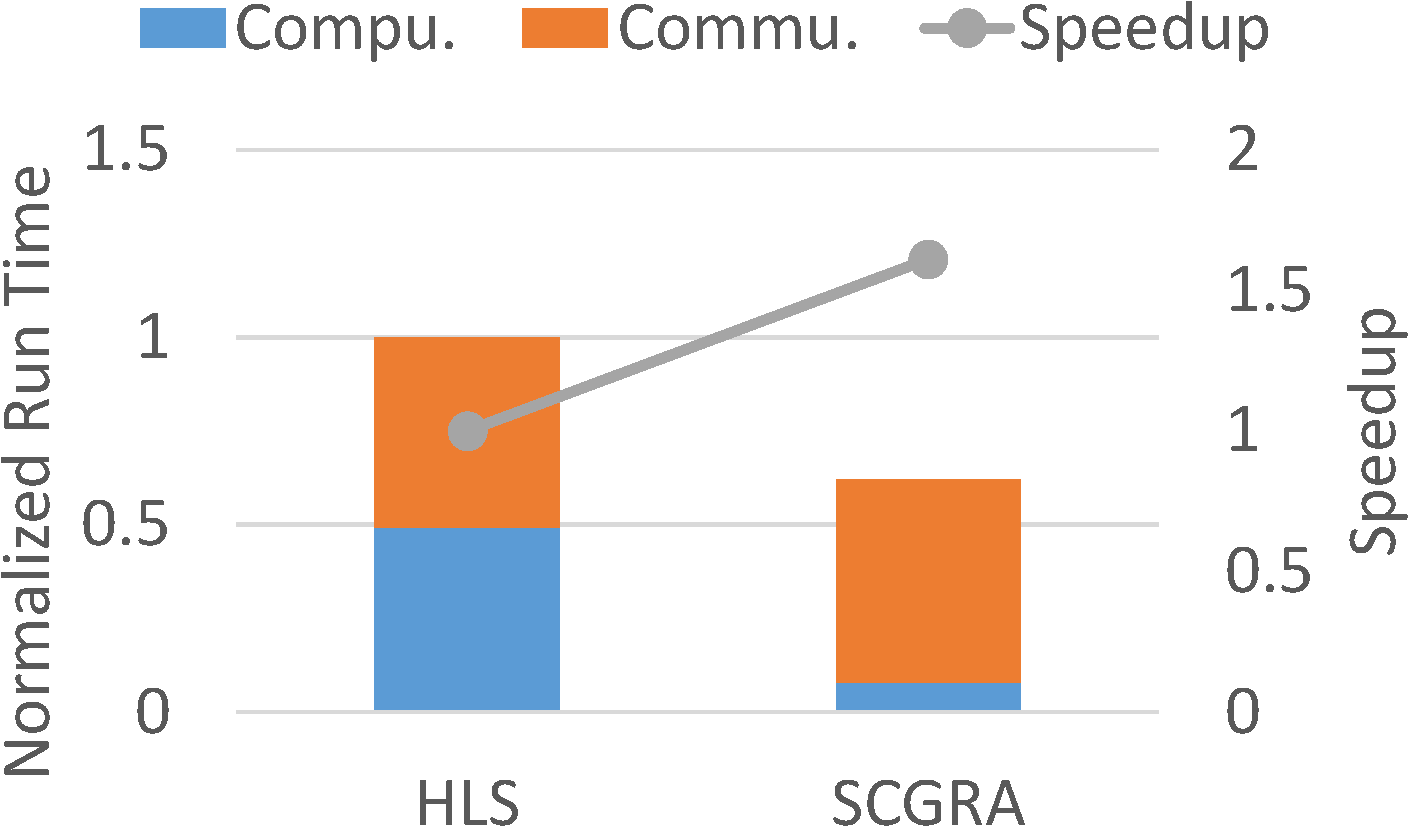
\includegraphics[width=0.22\textwidth]{km-hls-cp}
	}
    \caption{Performance comparison between the implementations 
        using HLS and the proposed automatic customization framework.
    All the run time is normalized to that of the HLS based implementations.}
	\label{fig:hls-cp}
\end{figure}


\figref{fig:hls-cp} shows the performance of the implementations using 
both design tools. The proposed customization framework utilizes 
SCGRA overlay as the backbone and it can't afford large 
BRAM for input/output buffers. As a result, the communication time is larger 
especially when there is a lot of data reuse between consecutive data transmission.
For instance, HLS based design can afford a 32k-word input buffer storing all 
the input data. However, the SCGRA overlay based design can only 
provide a 4k-word input buffer and it needs to transmit the same data 
multiple times to complete the matrix multiplication. Direct HLS can't support large 
loop unrolling due to the DSP resource constrain. SCGRA overlay based accelerator 
has a lot of distributed intermediate buffers and can accommodate larger loop unrolling.
Therefore, the accelerators generated using the proposed framework provides competitive 
pure computation time and overall performance especially for compute intensive loops.



\section{Limitations and Future Work}\label{sec:discussion}
While the current implementation of our proposed HLS methodology has demonstrated promising initial results, there are a number of limitations that must be acknowledged and possibly addressed in future work.

First and foremost, the proposed methodology is designed to synthesize parallel computing kernels to execute on FPGAs only. As such, it is not a generic methodology to perform HLS on random logic.  Furthermore, the proposed method is intended to serve as part of a larger HW/SW synthesis framework that targets hybrid CPU-FPGA systems. Therefore, many high-level design decisions such as the identification of compute kernel to offload to FPGAs are not handled in this work.

To maximize the amount of parallelism, loops are fully unrolled in the current implementation and thus the loop iterations in the kernels must be known at compile time. In the future, the degree of unrolling should be automatically determined based on the amount of available on chip resources. Since the scheduler depends on lock step execution, all the input data are assumed to be available whenever they are required and all the output data can always be accommodated by the store FIFO. As a result, the application with a large data set may require an extremely large input/output FIFO. In future, we may allow the SCGRA to be stalled to tolerate load/store latency variation and smaller load/store FIFO will be sufficient. 

Finally, on-chip ROM resources for instruction storage is our current resource limitation. We intend to alleviate this bottleneck in the future through the use of better instruction encoding schemes and instruction sequence reuse. Partial loop unrolling instead of fully loop unrolling as mentioned above will also help relieve this problem.

\section{Conclusions}\label{sec:conclusions}
In this paper, we have proposed a SCGRA based high-level synthesis (HLS) methodology for compiling computing kernels on FPGAs.  

By using an SCGRA as an intermediate compile step, the lengthy low-level implementation tool flow is reduced to a relatively rapid operation scheduling problem. The number of FPGA application debug cycles achievable per day is thus significantly increased, which contributes directly into higher application designers' productivity.

Despite the use of an additional layer of SCGRA on the target FPGA, the overall application performance is not necessarily compromised. Implementation with close to maximum clock frequency resulting from the highly regular structure of the SCGRA, in combination with an in-house scheduler that can effectively schedule operation to overlap with pipeline latencies are both contributing factors to such overall high performance. 

Compared to a conventional HLS methodology, experiments have shown that design compilation time is reduced by 10-100x while performance of the resulting application run time is improved by 0.8-21x.  The implementations resulting from the proposed HLS methodology consume more BRAMs but fewer SLICEs, LUTs, FFs and DSPs when compared to the conventional HLS implementations with relatively heavy loop unrolling.



\bibliographystyle{newapa}
\bibliography{refs}

\end{document}

